\documentclass[11pt]{article}

\usepackage[margin=1in]{geometry}
\usepackage[T1]{fontenc}
\usepackage[utf8]{inputenc}
\usepackage{lmodern}
\usepackage{microtype}
\usepackage{amsmath,amssymb,amsthm,mathtools}
\usepackage{bm}
\usepackage{booktabs,array,longtable}
\usepackage{hyperref}
\usepackage{xcolor}
\usepackage[most]{tcolorbox}
\usepackage{tikz}
\usepackage{pgfplots}
\usepackage{tikz-3dplot}
\usepackage{enumitem}
\usepackage{caption}
\usepackage{float}
\usepackage{fancyhdr}
\usepackage{titlesec}

\pgfplotsset{compat=1.18}
\usepgfplotslibrary{fillbetween}
\usetikzlibrary{arrows.meta,calc,intersections,patterns,decorations.pathreplacing,positioning,3d,backgrounds}

\hypersetup{
  colorlinks=true,
  linkcolor=blue!60!black,
  urlcolor=blue!60!black,
  citecolor=blue!60!black,
  pdftitle={Chapter 9. Linear Approximation, Tangent Planes, and Differentials}
}

\setlength{\headheight}{14pt}
\setlength{\parindent}{0pt}
\setlength{\parskip}{0.65em}
\setlist[itemize]{topsep=2pt,itemsep=2pt}
\setlist[enumerate]{topsep=2pt,itemsep=2pt}

\titleformat{\section}{\large\bfseries}{\thesection}{0.6em}{}
\titleformat{\subsection}{\normalsize\bfseries}{\thesubsection}{0.6em}{}

\pagestyle{fancy}
\fancyhf{}
\lhead{Chapter 9. Linear Approximation, Tangent Planes, and Differentials}
\rhead{\thepage}
\renewcommand{\headrulewidth}{0.4pt}

\newtcolorbox{chapteroverviewbox}{
  colback=blue!4,
  colframe=blue!50!black,
  boxrule=0.7pt,
  arc=2mm,
  left=2mm,right=2mm,top=1mm,bottom=1mm
}

\newtcolorbox{goalbox}{
  colback=green!4,
  colframe=green!45!black,
  title=Learning goals,
  fonttitle=\bfseries,
  boxrule=0.7pt,
  arc=2mm
}

\newtcolorbox{notebox}[1][]{
  colback=blue!3,
  colframe=blue!50!black,
  fonttitle=\bfseries,
  title=#1,
  boxrule=0.7pt,
  arc=2mm
}

\newtcolorbox{tipbox}[1][]{
  colback=green!3,
  colframe=green!45!black,
  fonttitle=\bfseries,
  title=#1,
  boxrule=0.7pt,
  arc=2mm
}

\newtcolorbox{importantbox}[1][]{
  colback=red!3,
  colframe=red!60!black,
  fonttitle=\bfseries,
  title=#1,
  boxrule=0.7pt,
  arc=2mm
}

\newtcolorbox{warningbox}[1][]{
  colback=yellow!8,
  colframe=orange!75!black,
  fonttitle=\bfseries,
  title=#1,
  boxrule=0.7pt,
  arc=2mm
}

\newtcbtheorem[number within=section]{examplebox}{Example}{
  enhanced,
  breakable,
  colback=white,
  colframe=blue!60!black,
  colbacktitle=blue!60!black,
  fonttitle=\bfseries,
  boxrule=0.7pt,
  arc=1.5mm,
  left=2mm,right=2mm,top=1mm,bottom=1mm
}{ex}

\newcommand{\R}{\mathbb R}
\newcommand{\grad}{\nabla}
\newcommand{\bx}{\mathbf{x}}
\newcommand{\ba}{\mathbf{a}}
\newcommand{\btheta}{\boldsymbol{\theta}}
\newcommand{\dd}{\,d}
\newcommand{\Var}{\operatorname{Var}}

\begin{document}

\begin{center}
  {\LARGE\bfseries Chapter 9. Linear Approximation, Tangent Planes, and Differentials\par}
  \vspace{0.3em}
  {\large The local linear model behind tangent planes, sensitivity, and uncertainty\par}
\end{center}

\begin{chapteroverviewbox}
The central message of this chapter is simple and powerful:
\[
\text{a differentiable multivariable function is approximately linear near a point.}
\]
In single-variable calculus, the tangent line is the best first-order approximation to a curve near a point. In multivariable calculus, the same idea becomes the \emph{tangent plane} for a graph $z=f(x,y)$ and the \emph{tangent hyperplane} for a function of many variables.

Algebraically, the approximation is built from partial derivatives. Geometrically, it is the flat object that best matches the surface near the point. Computationally, it is the first local model used in numerical methods, optimization, uncertainty propagation, and statistical approximation.
\end{chapteroverviewbox}

\begin{importantbox}[Core principle]
A differentiable multivariable function is approximately linear near a point.
\end{importantbox}

\begin{notebox}[Teaching-material connection]
This chapter develops tangent planes, linearization, differential approximation, differentiability, total differentials, and tangent planes to level surfaces. The examples $z=3x^2+y^2$, gradient-based approximation, and the level-surface problem $F(x,y,z)=x^3+y^2e^z+xyz$ are used as core models.
\end{notebox}

\begin{goalbox}
After studying this chapter, you should be able to:
\begin{enumerate}
  \item explain why tangent planes are multivariable tangent lines;
  \item find the tangent plane to a surface $z=f(x,y)$ at a point;
  \item compute the linearization $L(x,y)$ of a function $f(x,y)$ at $(a,b)$;
  \item use linearization to estimate nearby function values;
  \item write linear approximation in gradient-dot-product form;
  \item explain the difference between partial derivatives existing and differentiability;
  \item compute total differentials and use them for error propagation;
  \item find tangent planes to level surfaces $F(x,y,z)=c$;
  \item interpret local linear models in statistics, data science, and machine learning;
  \item use computation to visualize tangent planes and approximation errors.
\end{enumerate}
\end{goalbox}

\section{Review: tangent lines and local linearity}

For a single-variable function $y=f(x)$, the tangent line at $x=a$ is
\[
L(x)=f(a)+f'(a)(x-a).
\]
The tangent line is useful because when $x$ is close to $a$,
\[
f(x)\approx L(x).
\]
If $\Delta x=x-a$, then
\[
\Delta y=f(x)-f(a)\approx f'(a)\Delta x.
\]
The multivariable version is
\[
\Delta z\approx f_x(a,b)\Delta x+f_y(a,b)\Delta y.
\]
The right side is linear in the input changes $\Delta x$ and $\Delta y$.

\begin{figure}[H]
\centering
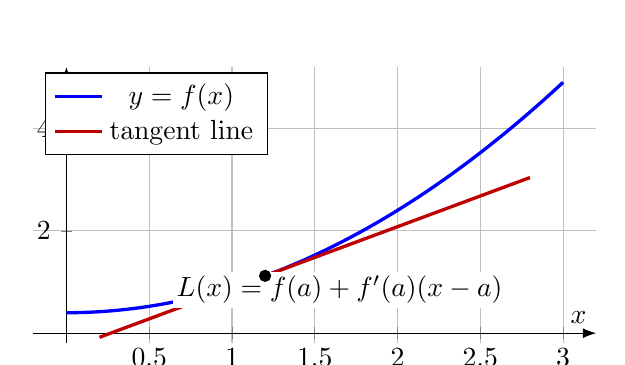
\begin{tikzpicture}
\begin{axis}[
  width=0.72\textwidth,
  height=0.42\textwidth,
  xmin=-0.2,xmax=3.2,
  ymin=-0.2,ymax=5.2,
  axis lines=middle,
  xlabel={$x$},ylabel={$y$},
  grid=both,
  axis line style={-Latex},
  legend style={at={(0.02,0.98)},anchor=north west,fill=white}
]
\addplot[very thick,blue,domain=0:3,samples=200] {0.5*x^2 + 0.4};
\addlegendentry{$y=f(x)$}
\addplot[very thick,red!75!black,domain=0.2:2.8] {1.2*(x-1.2)+1.12};
\addlegendentry{tangent line}
\addplot[only marks,mark=*,mark size=2pt] coordinates {(1.2,1.12)};
\node[fill=white,inner sep=1.5pt] at (axis cs:1.65,0.85) {$L(x)=f(a)+f'(a)(x-a)$};
\end{axis}
\end{tikzpicture}
\caption{In one variable, a tangent line is the local linear model. In two variables, the tangent line becomes a tangent plane.}
\end{figure}

\begin{tipbox}[Local does not mean global]
A tangent line or tangent plane usually gives a good approximation only near the point of tangency. Far away from the point, nonlinear curvature becomes important.
\end{tipbox}

\section{Tangent planes to graphs $z=f(x,y)$}

Let $z=f(x,y)$ be differentiable near $(a,b)$, and let
\[
P=(a,b,f(a,b))
\]
be the point on the graph. The tangent plane at $P$ is
\[
z-f(a,b)=f_x(a,b)(x-a)+f_y(a,b)(y-b).
\]
Equivalently,
\[
z=f(a,b)+f_x(a,b)(x-a)+f_y(a,b)(y-b).
\]
The function on the right is the \emph{linearization} of $f$ at $(a,b)$:
\[
L(x,y)=f(a,b)+f_x(a,b)(x-a)+f_y(a,b)(y-b).
\]
The approximation
\[
f(x,y)\approx L(x,y)
\]
is called the \emph{linear approximation} or \emph{tangent plane approximation}.

At the point $(a,b)$, the tangent plane matches three pieces of first-order information: the height $f(a,b)$, the $x$-direction slope $f_x(a,b)$, and the $y$-direction slope $f_y(a,b)$. A useful normal vector to the tangent plane is
\[
\langle f_x(a,b),f_y(a,b),-1\rangle.
\]

\section{Worked example: tangent plane to an elliptic paraboloid}

\begin{examplebox}{Tangent plane to $z=3x^2+y^2$}{paraboloidplane}
Find the tangent plane to
\[
z=f(x,y)=3x^2+y^2
\]
at the point $(1,2,7)$.

First check the height:
\[
f(1,2)=3(1)^2+(2)^2=7.
\]
The partial derivatives are
\[
f_x(x,y)=6x,\qquad f_y(x,y)=2y.
\]
At $(1,2)$,
\[
f_x(1,2)=6,\qquad f_y(1,2)=4.
\]
Therefore the tangent plane is
\[
z-7=6(x-1)+4(y-2),
\]
or
\[
z=6x+4y-7.
\]
Thus the linearization is
\[
L(x,y)=6x+4y-7.
\]
To estimate $f(1.1,1.9)$,
\[
L(1.1,1.9)=6(1.1)+4(1.9)-7=7.2.
\]
The exact value is
\[
f(1.1,1.9)=3(1.1)^2+(1.9)^2=7.24.
\]
\end{examplebox}

\begin{figure}[H]
\centering
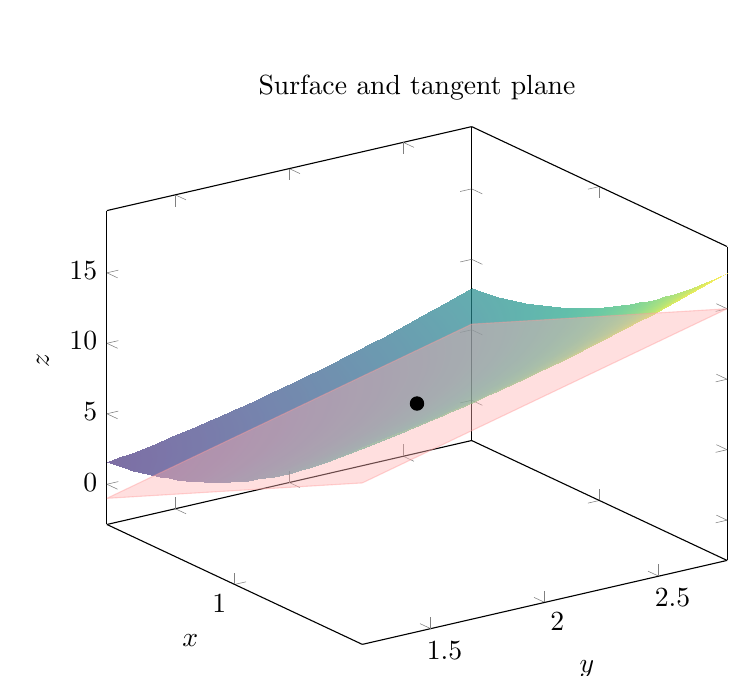
\begin{tikzpicture}
\begin{axis}[
  width=0.78\textwidth,
  view={55}{25},
  xlabel={$x$},ylabel={$y$},zlabel={$z$},
  domain=0.2:1.8, y domain=1.2:2.8,
  samples=30,samples y=30,
  z buffer=sort,
  colormap/viridis,
  title={Surface and tangent plane}
]
\addplot3[surf,shader=interp,opacity=0.7] {3*x^2 + y^2};
\addplot3[surf,shader=flat,opacity=0.42,draw=red!40,fill=red!30,domain=0.2:1.8,y domain=1.2:2.8,samples=2,samples y=2] {6*x + 4*y - 7};
\addplot3[only marks,mark=*,mark size=2.4pt] coordinates {(1,2,7)};
\end{axis}
\end{tikzpicture}
\caption{The graph of $z=3x^2+y^2$ and its tangent plane $z=6x+4y-7$ at $(1,2,7)$.}
\end{figure}

\section{Linear approximation in gradient form}

Let
\[
\Delta x=x-a,\qquad \Delta y=y-b,\qquad \Delta \mathbf{x}=\langle \Delta x,\Delta y\rangle.
\]
Then
\[
f(x,y)-f(a,b)\approx \grad f(a,b)\cdot \Delta \mathbf{x}.
\]
Equivalently,
\[
\Delta z\approx \grad f(a,b)\cdot \Delta \mathbf{x}.
\]
For a function $f:\R^n\to\R$, the same formula is
\[
f(\mathbf{x})\approx f(\mathbf{a})+\grad f(\mathbf{a})\cdot(\mathbf{x}-\mathbf{a}).
\]

\begin{examplebox}{Gradient-dot-displacement estimate}{graddot}
Suppose
\[
f(2,1)=13,\qquad \grad f(2,1)=\langle 12,2\rangle.
\]
Estimate $f(2.1,0.9)$.

The input displacement is
\[
\Delta \mathbf{x}=\langle 2.1-2,0.9-1\rangle=\langle 0.1,-0.1\rangle.
\]
Therefore
\[
\Delta z\approx \langle 12,2\rangle\cdot \langle 0.1,-0.1\rangle
=12(0.1)+2(-0.1)=1.
\]
So
\[
f(2.1,0.9)\approx 13+1=14.
\]
\end{examplebox}

\begin{figure}[H]
\centering
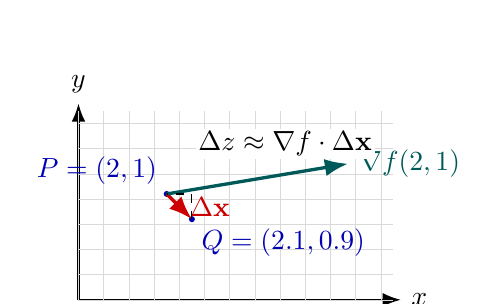
\begin{tikzpicture}[scale=3.2,>=Latex]
  \draw[->,thick] (0,0)--(1.28,0) node[right] {$x$};
  \draw[->,thick] (0,0)--(0,0.78) node[above] {$y$};
  \draw[help lines,gray!30,step=0.1] (0,0) grid (1.25,0.75);
  \coordinate (P) at (0.35,0.42);
  \coordinate (Q) at (0.45,0.32);
  \fill[blue!70!black] (P) circle (0.012) node[above left] {$P=(2,1)$};
  \fill[blue!70!black] (Q) circle (0.012) node[below right] {$Q=(2.1,0.9)$};
  \draw[->,very thick,red!80!black] (P)--(Q) node[midway,right] {$\Delta\mathbf{x}$};
  \draw[->,very thick,teal!70!black] (P)--++(0.72,0.12) node[right] {$\grad f(2,1)$};
  \draw[dashed] (Q)--++(0,0.10)--++(-0.10,0);
  \node[fill=white,inner sep=1pt] at (0.82,0.62) {$\Delta z\approx \grad f\cdot\Delta\mathbf{x}$};
\end{tikzpicture}
\caption{Linear approximation uses the dot product of the gradient and the displacement vector.}
\end{figure}

\section{Approximation error and curvature}

The linearization keeps only first-order information. The error comes from second-order and higher-order behavior. For
\[
f(x,y)=3x^2+y^2,
\]
the tangent plane at $(1,2)$ is
\[
L(x,y)=6x+4y-7.
\]
The error is
\[
E(x,y)=f(x,y)-L(x,y)=3(x-1)^2+(y-2)^2.
\]
This is always nonnegative because the surface is convex and lies above its tangent plane. The error is small near $(1,2)$ and grows quadratically as we move away.

\begin{figure}[H]
\centering
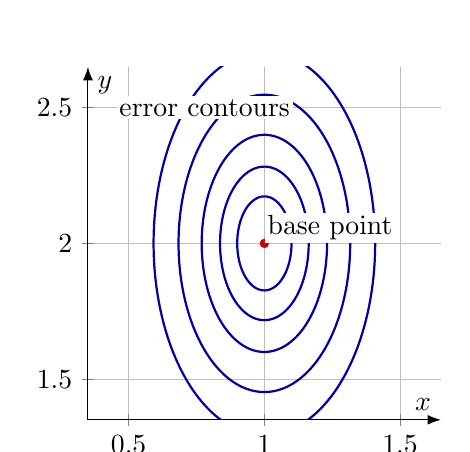
\begin{tikzpicture}
\begin{axis}[
  width=0.62\textwidth,
  height=0.5\textwidth,
  xmin=0.35,xmax=1.65,
  ymin=1.35,ymax=2.65,
  axis equal image,
  axis lines=middle,
  xlabel={$x$},ylabel={$y$},
  grid=both,
  axis line style={-Latex}
]
\foreach \c/\lab in {0.03/{},0.08/{},0.16/{},0.30/{},0.50/{}}{
  \addplot[domain=0:360,samples=240,blue!65!black,thick] ({1+sqrt(\c/3)*cos(x)},{2+sqrt(\c)*sin(x)});
}
\fill[red!80!black] (axis cs:1,2) circle (1.7pt);
\node[above right,fill=white,inner sep=1pt] at (axis cs:1,2) {base point};
\node[fill=white,inner sep=1pt] at (axis cs:0.78,2.50) {error contours};
\end{axis}
\end{tikzpicture}
\caption{The linearization error is small near the base point and grows quadratically as we move away.}
\end{figure}

\begin{notebox}[Connection to later approximation]
Taylor approximation makes this precise. The second-order term involves the Hessian matrix. Linear approximation is first-order Taylor approximation; quadratic approximation is second-order Taylor approximation.
\end{notebox}

\section{Differentiability}

A function $f(x,y)$ is \emph{differentiable} at $(a,b)$ if its change can be written as a linear part plus an error that becomes negligible compared with the size of the input change. One way to state this is
\[
\Delta z=f_x(a,b)\Delta x+f_y(a,b)\Delta y+\varepsilon_1\Delta x+\varepsilon_2\Delta y,
\]
where
\[
\varepsilon_1\to 0,\qquad \varepsilon_2\to 0
\]
as $(\Delta x,\Delta y)\to (0,0)$. Equivalently,
\[
f(a+\Delta x,b+\Delta y)=f(a,b)+f_x(a,b)\Delta x+f_y(a,b)\Delta y+\text{small error}.
\]
The important idea is not just that the partial derivatives exist. The important idea is that together they produce a good linear model near the point.

\begin{warningbox}[Partial derivatives alone are not enough]
A function may have partial derivatives at a point but fail to be differentiable there. Differentiability is stronger than the existence of coordinate-direction slopes.
\end{warningbox}

\begin{tipbox}[Sufficient condition for differentiability]
If $f_x$ and $f_y$ exist near $(a,b)$ and are continuous at $(a,b)$, then $f$ is differentiable at $(a,b)$.
\end{tipbox}

\section{A cautionary example}

Consider
\[
f(x,y)=
\begin{cases}
\dfrac{xy}{\sqrt{x^2+y^2}}, & (x,y)\ne (0,0),\\[0.6em]
0, & (x,y)=(0,0).
\end{cases}
\]
At the origin, the coordinate partial derivatives exist:
\[
f_x(0,0)=0,\qquad f_y(0,0)=0.
\]
So the candidate linearization is $L(x,y)=0$. However, along the line $y=x$,
\[
f(x,x)=\frac{x^2}{\sqrt{2x^2}}=\frac{|x|}{\sqrt2}.
\]
This is not negligible compared with the distance $\sqrt{x^2+x^2}=\sqrt2|x|$. Therefore the function is not differentiable at the origin.

\begin{figure}[H]
\centering
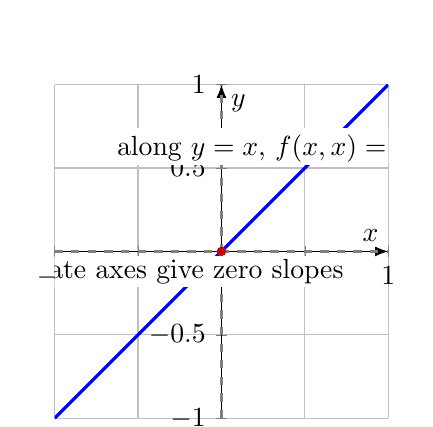
\begin{tikzpicture}
\begin{axis}[
  width=0.62\textwidth,
  height=0.48\textwidth,
  xmin=-1,xmax=1,
  ymin=-1,ymax=1,
  axis equal image,
  axis lines=middle,
  xlabel={$x$},ylabel={$y$},
  grid=both,
  axis line style={-Latex}
]
\addplot[very thick,blue,domain=-1:1,samples=200] {x};
\addplot[thick,gray,dashed] coordinates {(-1,0) (1,0)};
\addplot[thick,gray,dashed] coordinates {(0,-1) (0,1)};
\node[fill=white,inner sep=1pt] at (axis cs:0.45,0.63) {along $y=x$, $f(x,x)=|x|/\sqrt2$};
\node[fill=white,inner sep=1pt] at (axis cs:-0.42,-0.12) {coordinate axes give zero slopes};
\fill[red!80!black] (axis cs:0,0) circle (1.7pt);
\end{axis}
\end{tikzpicture}
\caption{A function can have coordinate partial derivatives at a point but still fail to be differentiable there.}
\end{figure}

\section{Tangent planes to level surfaces}

Many important surfaces are not given as graphs $z=f(x,y)$. Instead, they are given implicitly as level surfaces
\[
F(x,y,z)=c.
\]
Suppose $P=(a,b,c_0)$ is a point on the level surface. If
\[
\grad F(P)\ne \mathbf 0,
\]
then the gradient vector is normal to the level surface at $P$. Therefore the tangent plane is
\[
\grad F(P)\cdot \langle x-a,y-b,z-c_0\rangle=0.
\]
In coordinates, if
\[
\grad F(P)=\langle F_x(P),F_y(P),F_z(P)\rangle,
\]
then the tangent plane is
\[
F_x(P)(x-a)+F_y(P)(y-b)+F_z(P)(z-c_0)=0.
\]

If a curve $\mathbf r(t)$ lies on the level surface, then $F(\mathbf r(t))=c$. Differentiating with respect to $t$ gives
\[
\grad F(\mathbf r(t))\cdot \mathbf r'(t)=0.
\]
Thus the gradient is perpendicular to every tangent direction on the surface.

\begin{figure}[H]
\centering
\tdplotsetmaincoords{70}{115}
\begin{tikzpicture}[tdplot_main_coords,scale=1.25,>=Latex]
  \coordinate (P) at (0,0,0);
  \filldraw[fill=blue!12,draw=blue!60!black,opacity=0.9] (-2,-1,0)--(2,-1,0)--(2,1,0)--(-2,1,0)--cycle;
  \draw[->,very thick,red!80!black] (P)--(0,0,2.2) node[right] {$\grad F(P)$};
  \draw[->,thick,teal!80!black] (P)--(1.4,0.45,0) node[below] {tangent direction};
  \draw[->,thick,teal!80!black] (P)--(-0.4,1.1,0) node[left] {tangent direction};
  \fill[red!80!black] (P) circle (1.5pt) node[below right] {$P$};
  \node[blue!60!black] at (0,-1.25,0) {tangent plane};
\end{tikzpicture}
\caption{For a level surface, the gradient $\nabla F(P)$ is normal to the tangent plane.}
\end{figure}

\section{Worked example: linearization and tangent plane to a level surface}

\begin{examplebox}{Linearization and tangent plane for a level surface}{levelsurface}
Let
\[
F(x,y,z)=x^3+y^2e^z+xyz
\]
and let $P=(1,2,0)$.

First evaluate the function:
\[
F(1,2,0)=1^3+2^2e^0+1\cdot 2\cdot 0=5.
\]
The partial derivatives are
\[
F_x=3x^2+yz,
\]
\[
F_y=2ye^z+xz,
\]
\[
F_z=y^2e^z+xy.
\]
At $P=(1,2,0)$,
\[
F_x(P)=3,\qquad F_y(P)=4,\qquad F_z(P)=6.
\]
So the linearization is
\[
L(x,y,z)=5+3(x-1)+4(y-2)+6z.
\]
Equivalently,
\[
L(x,y,z)=3x+4y+6z-6.
\]
Now estimate:
\[
F(1.1,1.9,0)\approx L(1.1,1.9,0)=3(1.1)+4(1.9)-6=4.9.
\]
The level surface through $P$ is $F(x,y,z)=5$. Its tangent plane is
\[
3(x-1)+4(y-2)+6z=0,
\]
or
\[
3x+4y+6z-11=0.
\]
\end{examplebox}

\section{Total differentials}

For a differentiable function $z=f(x,y)$, define $dx$ and $dy$ as independent small changes in the input variables. The \emph{total differential} is
\[
dz=f_x(x,y)\,dx+f_y(x,y)\,dy.
\]
At a specific point $(a,b)$, this becomes
\[
dz=f_x(a,b)\,dx+f_y(a,b)\,dy.
\]
The differential is the linear approximation to the actual change:
\[
\Delta z\approx dz.
\]
For a function of three variables $w=f(x,y,z)$,
\[
dw=f_x\,dx+f_y\,dy+f_z\,dz.
\]
More generally, for $f:\R^n\to\R$,
\[
df=\grad f(\mathbf{x})\cdot d\mathbf{x}.
\]

\begin{notebox}[Why differentials matter]
Deltas such as $\Delta x$ and $\Delta y$ represent actual changes. Differentials such as $dx$ and $dy$ are independent input changes used in the linear model. The differential $dz$ is the predicted output change from the tangent plane.
\end{notebox}

\section{Error propagation and sensitivity analysis}

In applied problems, inputs are often measured with error. Linear approximation estimates how input error affects output error. Suppose
\[
z=f(x,y)
\]
and the possible measurement errors are
\[
|dx|\le \epsilon_x,\qquad |dy|\le \epsilon_y.
\]
Then a first-order estimate for the output error is
\[
|dz|\le |f_x(x,y)|\epsilon_x+|f_y(x,y)|\epsilon_y.
\]
If $dx$ and $dy$ are random errors with covariance matrix $\Sigma$, then the approximate variance of the output is
\[
\Var(df)\approx \grad f(\mathbf{x})^T\Sigma\grad f(\mathbf{x}).
\]
This is the core idea behind the delta method in statistics.

\begin{examplebox}{Volume of a cylinder}{cylindervolume}
The volume of a cylinder is
\[
V(r,h)=\pi r^2h.
\]
The differential is
\[
dV=2\pi rh\,dr+\pi r^2\,dh.
\]
At $r=3$ and $h=10$,
\[
dV=60\pi\,dr+9\pi\,dh.
\]
If $dr=0.02$ and $dh=-0.05$, then
\[
dV\approx 60\pi(0.02)+9\pi(-0.05)=0.75\pi\approx 2.36.
\]
\end{examplebox}

\begin{figure}[H]
\centering
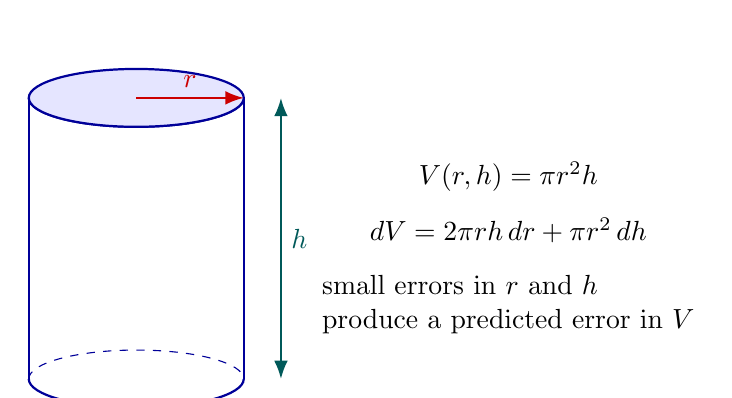
\begin{tikzpicture}[scale=1.05,>=Latex]
  \draw[fill=blue!10,draw=blue!60!black,thick] (-1.3,1.7) arc[start angle=180,end angle=360,x radius=1.3,y radius=0.35];
  \draw[fill=blue!10,draw=blue!60!black,thick] (0,1.7) ellipse (1.3 and 0.35);
  \draw[thick,blue!60!black] (-1.3,1.7)--(-1.3,-1.7);
  \draw[thick,blue!60!black] (1.3,1.7)--(1.3,-1.7);
  \draw[thick,blue!60!black] (-1.3,-1.7) arc[start angle=180,end angle=360,x radius=1.3,y radius=0.35];
  \draw[dashed,blue!60!black] (-1.3,-1.7) arc[start angle=180,end angle=0,x radius=1.3,y radius=0.35];
  \draw[->,red!80!black,thick] (0,1.7)--(1.3,1.7) node[midway,above] {$r$};
  \draw[<->,teal!70!black,thick] (1.75,-1.7)--(1.75,1.7) node[midway,right] {$h$};
  \node at (4.5,0.75) {$V(r,h)=\pi r^2h$};
  \node at (4.5,0.1) {$dV=2\pi rh\,dr+\pi r^2\,dh$};
  \node[align=left] at (4.5,-0.8) {small errors in $r$ and $h$\\produce a predicted error in $V$};
\end{tikzpicture}
\caption{Linear error propagation predicts how measurement errors in radius and height affect cylinder volume.}
\end{figure}

\section{Linearization as a local model in statistics and machine learning}

Many statistical and machine-learning models depend on parameters. A simple example is a two-parameter linear prediction model
\[
\widehat y=\beta_0+\beta_1x.
\]
A more complicated model may have many parameters:
\[
\widehat y=f(x;\theta_1,\theta_2,\ldots,\theta_n).
\]
Near a parameter vector $\btheta_0$, linear approximation gives
\[
f(x;\btheta)\approx f(x;\btheta_0)+\grad_{\btheta}f(x;\btheta_0)\cdot(\btheta-\btheta_0).
\]
This is the local linear model used in sensitivity analysis, uncertainty propagation, first-order optimization, local approximation of nonlinear regression models, and gradient-based learning.

\subsection*{Local linearization of a sigmoid}

The logistic sigmoid is
\[
\sigma(t)=\frac{1}{1+e^{-t}}.
\]
If $t=\beta_0+\beta_1x$, then
\[
p(x;\beta_0,\beta_1)=\sigma(\beta_0+\beta_1x).
\]
For fixed $x$, this is a function of the parameters $\beta_0$ and $\beta_1$. Its gradient tells how the predicted probability changes when the parameters change.

\begin{figure}[H]
\centering
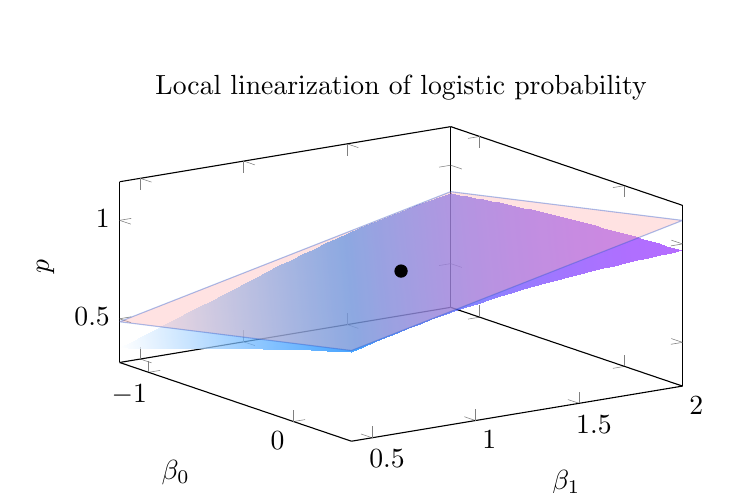
\begin{tikzpicture}
\begin{axis}[
  width=0.72\textwidth,
  height=0.46\textwidth,
  view={55}{28},
  xlabel={$\beta_0$},ylabel={$\beta_1$},zlabel={$p$},
  domain=-1.2:0.4, y domain=0.4:2.0,
  samples=30,samples y=30,
  z buffer=sort,
  colormap/cool,
  title={Local linearization of logistic probability}
]
\addplot3[surf,shader=interp,opacity=0.72] {1/(1+exp(-(x+1.5*y)))};
% tangent plane near beta0=-0.4, beta1=1.2, x0=1.5
\addplot3[surf,opacity=0.38,draw=red!40,fill=red!30,domain=-1.2:0.4,y domain=0.4:2.0,samples=2,samples y=2]
{0.8021839 + 0.1586849*(x+0.4) + 0.2380274*(y-1.2)};
\addplot3[only marks,mark=*,mark size=2.2pt] coordinates {(-0.4,1.2,0.8021839)};
\end{axis}
\end{tikzpicture}
\caption{A nonlinear probability model is locally approximated by its tangent plane in parameter space.}
\end{figure}

\section{Numerical linearization from finite differences}

In real applications, we may not have a symbolic formula for the gradient. We may only have a black-box function that can be evaluated. Then we can approximate the gradient numerically. For a function $f(x,y)$, central finite differences give
\[
f_x(a,b)\approx \frac{f(a+h,b)-f(a-h,b)}{2h},
\]
\[
f_y(a,b)\approx \frac{f(a,b+h)-f(a,b-h)}{2h}.
\]
Then the numerical linearization is
\[
L(x,y)=f(a,b)+\widehat f_x(a,b)(x-a)+\widehat f_y(a,b)(y-b).
\]

\begin{figure}[H]
\centering
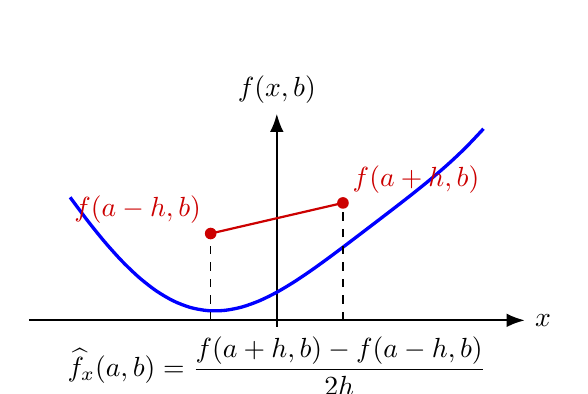
\begin{tikzpicture}[>=Latex,scale=1.05]
  \draw[->,thick] (-3,0)--(3,0) node[right] {$x$};
  \draw[->,thick] (0,-0.3)--(0,2.5) node[above] {$f(x,b)$};
  \draw[very thick,blue,domain=-2.5:2.5,smooth,variable=\t] plot ({\t},{0.3+0.25*(\t+0.4)^2+0.25*sin(80*\t)});
  \draw[dashed] (-0.8,0)--(-0.8,1.05);
  \draw[dashed] (0.8,0)--(0.8,1.42);
  \fill[red!80!black] (-0.8,1.05) circle (2pt) node[above left] {$f(a-h,b)$};
  \fill[red!80!black] (0.8,1.42) circle (2pt) node[above right] {$f(a+h,b)$};
  \draw[red!80!black,thick] (-0.8,1.05)--(0.8,1.42);
  \node[align=center,fill=white] at (0,-0.55) {$\displaystyle \widehat f_x(a,b)=\frac{f(a+h,b)-f(a-h,b)}{2h}$};
\end{tikzpicture}
\caption{Finite differences approximate the gradient used in a local linear model.}
\end{figure}

\section{Vector-valued and matrix viewpoints}

The scalar-valued formula
\[
f(\mathbf{x})\approx f(\mathbf{a})+\grad f(\mathbf{a})\cdot(\mathbf{x}-\mathbf{a})
\]
has a natural extension to vector-valued functions. If
\[
\mathbf F:\R^n\to\R^m,
\]
then the best first-order approximation is
\[
\mathbf F(\mathbf{x})\approx \mathbf F(\mathbf{a})+J_{\mathbf F}(\mathbf{a})(\mathbf{x}-\mathbf{a}),
\]
where $J_{\mathbf F}(\mathbf{a})$ is the \emph{Jacobian matrix}. The key idea is that derivatives in many variables are linear maps. The gradient-dot-product formula is the scalar-output version of this principle.

\section{Common mistakes}

\begin{warningbox}[Mistake 1: using the wrong base point]
The tangent plane formula must use the point of tangency $(a,b)$ and the height $f(a,b)$. Do not plug in the nearby point where you want the estimate.
\end{warningbox}

\begin{warningbox}[Mistake 2: mixing up graph surfaces and level surfaces]
For a graph $z=f(x,y)$, use
\[
z-f(a,b)=f_x(a,b)(x-a)+f_y(a,b)(y-b).
\]
For a level surface $F(x,y,z)=c$, use
\[
\grad F(P)\cdot \langle x-a,y-b,z-c_0\rangle=0.
\]
\end{warningbox}

\begin{warningbox}[Mistake 3: thinking partial derivatives guarantee differentiability]
Partial derivatives measure coordinate-direction slopes. Differentiability means there is a good linear approximation in all directions at once.
\end{warningbox}

\section{Summary of key formulas}

For $z=f(x,y)$:
\[
L(x,y)=f(a,b)+f_x(a,b)(x-a)+f_y(a,b)(y-b).
\]
Tangent plane to $z=f(x,y)$:
\[
z-f(a,b)=f_x(a,b)(x-a)+f_y(a,b)(y-b).
\]
Gradient form:
\[
f(x,y)-f(a,b)\approx \grad f(a,b)\cdot \langle x-a,y-b\rangle.
\]
Total differential:
\[
dz=f_x\,dx+f_y\,dy.
\]
For $f:\R^n\to\R$:
\[
f(\mathbf{x})\approx f(\mathbf{a})+\grad f(\mathbf{a})\cdot(\mathbf{x}-\mathbf{a}).
\]
Tangent plane to $F(x,y,z)=c$ at $P=(a,b,c_0)$:
\[
F_x(P)(x-a)+F_y(P)(y-b)+F_z(P)(z-c_0)=0.
\]

\section{Practice problems}

\subsection*{Conceptual problems}
\begin{enumerate}
  \item In your own words, explain why a tangent plane is a local linear model.
  \item What information does the tangent plane to $z=f(x,y)$ match at the base point?
  \item Explain why the gradient of $F$ is normal to the level surface $F(x,y,z)=c$.
  \item Explain the difference between $\Delta z$ and $dz$.
  \item Why can a function have partial derivatives but fail to be differentiable?
\end{enumerate}

\subsection*{Skill problems}
\begin{enumerate}[start=6]
  \item Find the tangent plane to $z=x^2+3y^2$ at $(1,-1,4)$.
  \item Find the linearization of $f(x,y)=e^{xy}+x^2y$ at $(1,0)$.
  \item Use a linear approximation to estimate $\sqrt{(4.1)^2+(2.9)^2}$.
  \item Suppose $f(3,2)=10$ and $\grad f(3,2)=\langle -2,5\rangle$. Estimate $f(2.9,2.2)$.
  \item Find $dz$ for $z=x^2\sin y+e^{xy}$.
\end{enumerate}

\subsection*{Level-surface problems}
\begin{enumerate}[start=11]
  \item Find the tangent plane to $x^2+y^2+z^2=14$ at $(1,2,3)$.
  \item Find the tangent plane to $x^3+y^2e^z+xyz=5$ at $(1,2,0)$.
  \item Find the tangent plane to $\ln(x+y+z)=0$ at $(1,0,0)$.
  \item Find a normal vector to the level surface $F(x,y,z)=x^2y+yz^2$ at $(1,2,1)$.
  \item Find the linearization of $F(x,y,z)=x^2+y^2+z^2$ at $(1,2,2)$.
\end{enumerate}

\subsection*{Applied and computational problems}
\begin{enumerate}[start=16]
  \item The volume of a rectangular box is $V=xyz$. Use differentials to estimate the change in volume when $(x,y,z)=(10,5,2)$ changes by $(dx,dy,dz)=(0.1,-0.05,0.02)$.
  \item The BMI formula is $B(W,H)=703W/H^2$, where $W$ is weight in pounds and $H$ is height in inches. Use differentials to estimate how small errors in $W$ and $H$ affect BMI.
  \item For $f(x,y)=\sin(xy)+x^2$, use finite differences to estimate the tangent plane at $(1,1)$.
  \item For a prediction model $p(\beta_0,\beta_1)=1/(1+e^{-(\beta_0+2\beta_1)})$, find the linearization at $(0,1)$.
  \item Choose a nonlinear function of two variables, plot the surface and tangent plane, and describe where the approximation is accurate.
\end{enumerate}

\section{Python lab and interactive page}

The Python lab for this chapter should ask students to build local linear models from symbolic formulas, numerical finite differences, and data-based approximations. Recommended lab activities:
\begin{enumerate}
  \item visualize the surface $z=3x^2+y^2$ and its tangent plane at $(1,2)$;
  \item compare exact values with linearized values on a grid;
  \item compute and visualize approximation error;
  \item estimate gradients numerically using finite differences;
  \item find tangent planes to level surfaces using gradients;
  \item simulate error propagation for measurement uncertainty;
  \item explore local linearization of a logistic probability model.
\end{enumerate}

Resources:
\begin{itemize}
  \item Notebook lab: Chapter 9 linear approximation lab.
  \item Interactive HTML page: \texttt{chapter-09.html}.
\end{itemize}

\section{Chapter summary}

Linear approximation is the first major synthesis point of multivariable calculus. Partial derivatives become a gradient. The gradient becomes a local linear model. The local linear model becomes a tangent plane, a differential, a sensitivity estimate, and a computational approximation.

For graphs $z=f(x,y)$, the tangent plane is
\[
z=f(a,b)+f_x(a,b)(x-a)+f_y(a,b)(y-b).
\]
For level surfaces $F(x,y,z)=c$, the tangent plane is determined by the normal vector $\grad F(P)$:
\[
\grad F(P)\cdot(\mathbf{x}-P)=0.
\]
In applied mathematics and statistics, this chapter is the foundation for error propagation, the delta method, local optimization, and first-order approximation of nonlinear models. In machine learning and AI, it is the idea behind using gradients to approximate and improve complicated models one small step at a time.

\end{document}
